\documentclass[12pt]{amsart}
\usepackage{style,graphicx}

\author{Ann Clifton}
\address{Lafayette College}
\title[Exam 1]{Exam 1\\Math 186}
\date{February 20, 2019}

\begin{document}
\maketitle

\begin{center}
  \fbox{\fbox{\parbox{5.5in}{\centering
        \noindent Answer the questions in the spaces provided on the
        question sheets and turn them in at the end of the exam period.\\


        \noindent It is advised, although not required, that you check your answers.
        All supporting work is required.
        Unsupported or otherwise mysterious answers will \textbf{not receive credit.}\\
        
        \noindent You may use a calculator but you may {\bf not} use any other electronic device, including cell phones, smart watches, etc.\\
        
        \noindent By writing your name on the line below, you indicate that you have read and understand these directions.
       }}}
\end{center}

\vspace{0.2in}
\makebox[\textwidth]{Name:\enspace\hrulefill}
\vspace{.3in}




\theoremstyle{definition}
\newtheorem{thm}{}
\renewcommand{\qedsymbol}{}

Remember: This exam has no impact on your worth as a human being.  You got this!!!
\vspace{.3in}
\begin{center}
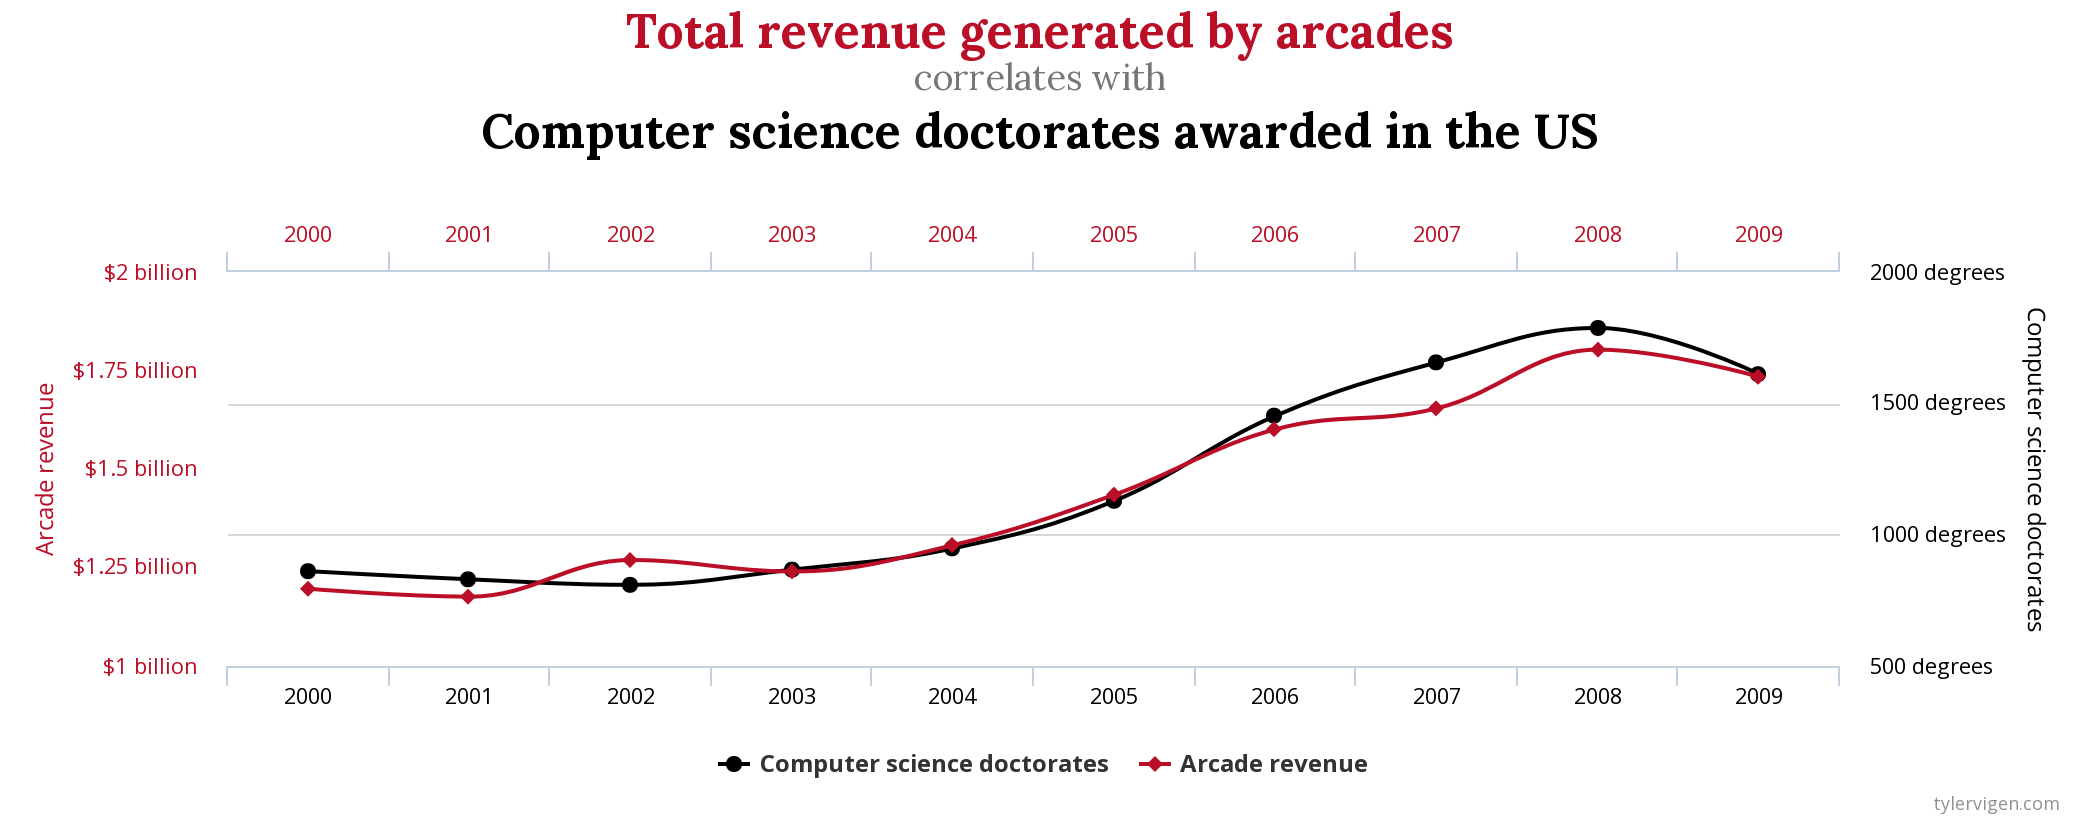
\includegraphics[scale=.25]{chart.png}
\end{center}



\newpage




\begin{thm} (10 points)
Let's talk about last night's Oscars!  Suppose we're interested in seeing whether a movie's Rotten Tomatoes rating is a good predictor of how many Oscar nominations it will receive.  The data for the nominees for Best Picture are below.
\begin{center}
$\begin{array}{|c|c|c|}
\hline
\text{{\bf Movie}}&\text{\bf{Rotten Tomatoes Rating}}&\text{\bf{\# of Oscar Nominations}}\\ 
\hline
\text{Black Panther}& 97 & 7\\
\hline
\text{BlacKkKlansman}& 96 & 6\\
\hline
\text{Bohemian Rhapsody} & 61 & 5\\
\hline
\text{The Favourite} & 94 & 10\\
\hline
\text{Green Book} & 80 & 5\\
\hline
\text{Roma} & 96 & 10\\
\hline
\text{A Star is Born} & 90 & 8\\
\hline
\text{Vice} & 66 & 8\\
\hline
\end{array}$
\end{center}

\begin{itemize}
\item[(a)] Explain why a scatterplot would be an appropriate display for this data.  What are the explanatory and response variables?

\vspace{1.5in}

\item[(b)] The least-squares regression line for this data is given by $y=1.938+0.064x$.  Interpret the slope and $y$-intercept in the context of the problem.

\vspace{1in}

\item[(c)] There is a list of 32 films on Wikipedia that have all received a 0\% rating on Rotten Tomatoes.  Would it be wise to use the model in part (b) to predict the number of Oscar nominations for a film with such a rating? Why or why not?

\vspace{1in}

\item[(d)] The correlation value for this data set is $r=0.4619$.  What percentage of the variation in Emmy nominations can be explained by the Rotten Tomatoes rating? Do you think that the Rotten Tomatoes rating is a good predictor of Emmy nominations? Why or why not?
\end{itemize}
\end{thm}

\newpage

\begin{thm} (10 points) In a class with a recent exam, both you and a classmate forgot to put your names on the papers.  After the professor hands back all of the papers with names, she is left with just two.  She tells you that the distribution of exam scores was bell-shaped, and that the score on the first unnamed exam was the $70^{\text{th}}$ percentile, while the score on the second was one standard deviation above the mean.  Which one do you hope is yours and why?
\end{thm}

\vspace{3in}

\begin{thm} (10 points) Through accounting procedures, it is known that about 10\% of the employees in a store are stealing.  The managers would like to fire the thieves, but their only tool in distinguishing them from the honest employees is a lie detector test that is only 90\% accurate.  That is, if an employee is a thief, he or she will fail the test with probability 0.9, and if an employee is not a thief, he or she will pass the test with probability 0.9.  If an employee fails the test, what is the probability that he or she is a thief?
\end{thm}

\newpage

\begin{thm} (10 points) The following contingency table/two-way table classifies the members of a certain government into political party (Liberal or Conservative) and whether they support or oppose the spending bill that is currently up for adoption.
\begin{center}
$\begin{array}{l|cc|c}
& {\text{\bf Support}} & {\text{\bf Oppose}} & {\text{\bf Total}}\\ \hline
{\text{\bf Liberal}} & 47 & 11 & 58 \\
{\text{\bf Conservative}} & 14 & 35 & 49\\ \hline
{\text{\bf Total}} & 61 & 46 & 107\\
\end{array}$
\end{center}
Imagine randomly selecting one member of the government.  Let $L$, $C$, $S$, and $O$ denote the events of selecting a liberal, a conservative, a bill supporter, and a bill opposer, respectively.  
\begin{itemize}
\item[(a)]  Find $P(C{\text{ and }}S)$.
\vspace{1in}
\item[(b)] Find $P(S\vert L)$.
\end{itemize}
\end{thm}

\vspace{.8in}

\begin{thm} (10 points) A five-number summary for the heights in inches of the women who participated in a survey is below:
\begin{center}
{\bf Female Heights\\ (inches)}\\
$\begin{array}{cccc}\hline
{\text{\bf{Median}}} & & 65& \\
{\text{\bf{Quartiles}}} & 63.5 & & 67.5 \\
{\text{\bf{Extremes}}} & 59 & & 71\\
\end{array}$
\end{center}
\begin{itemize}
\item[(a)] What is the range of heights?

\vspace{1in}

\item[(b)] What is the range of heights containing the shortest one-fourth of the women?

\vspace{1in}

\item[(c)] Are there any outliers? How do you know?

\end{itemize}
\end{thm}






\end{document}
